\usetheme{FINKI}
\usepackage{thumbpdf}
\usepackage{wasysym}
\usepackage{ucs}
\usepackage[T2A]{fontenc}
\usepackage[utf8]{inputenc}
\usepackage{pgf,pgfarrows,pgfnodes,pgfautomata,pgfheaps,pgfshade}
\usepackage{verbatim}
\usepackage{listings}
\usepackage{fancybox} 



\pdfinfo
{
  /Title       (AV7)
  /Creator     (Tomche Delev)
  /Author      (Tomche Delev)
}


\title[АВ7]{Аудиториски вежби 7}
\subtitle{Контрола на верзии\\Системи за контрола на верзии (SVN) }
\author{Основи на софтверско инженерство}
\date{}
\pgfdeclareimage[width=0.6\paperwidth]{finki_logo}{finki_name}
\titlegraphic{\pgfuseimage{finki_logo}}



\begin{document}

\frame[plain]{\titlepage}

%Automatic table of contents
\section*{}
\begin{frame}
  \frametitle{Содржина}
  \tableofcontents[section=1,hidesubsections]
\end{frame}

\AtBeginSection[]
{
  \frame<handout:0>
  {
    \frametitle{Содржина}
    \tableofcontents[currentsection,hideallsubsections]
  }
}

\AtBeginSubsection[]
{
  \frame<handout:0>
  {
    \frametitle{Содржина}
    \tableofcontents[sectionstyle=show/hide,subsectionstyle=show/shaded/hide]
  }
}

\newcommand<>{\highlighton}[1]{%
  \alt#2{\structure{#1}}{{#1}}
}

\newcommand{\icon}[1]{\pgfimage[height=1em]{#1}}

\lstset{language=C,captionpos=b,
tabsize=4,frame=lines,
basicstyle=\scriptsize\ttfamily,
keywordstyle=\color{blue},
commentstyle=\color{lightgray},
stringstyle=\color{violet},
breaklines=true,showstringspaces=false}

%%%%%%%%%%%%%%%%%%%%%%%%%%%%%%%%%%%%%%%%%
%%%%%%%%%% Content starts here %%%%%%%%%%
%%%%%%%%%%%%%%%%%%%%%%%%%%%%%%%%%%%%%%%%%
\section{Што е тоа контрола на верзии?}

\begin{frame}{Контрола на верзии}
\begin{itemize}
\item Што е тоа контрола на верзии?
    \begin{itemize}
    \item Контрола на верзии претставува управување со промените на документи,
    \textbf{изворни програми} или други информации зачувани како компјутерски датотеки.
    \end{itemize}
\item Зошто ни треба?
    \begin{itemize}
    \item Ако направиме некоја грешка или едноставно сакаме да се
    вратиме на некоја претходна верзија на документот.
    \end{itemize}
\item Каде се употребува?
    \begin{itemize}
    \item Најчесто се употребува во развојот на софтвер, каде што тим од луѓе може да ја менуваат истата датотека.
    \end{itemize}
\end{itemize}
\end{frame}

\begin{frame}[fragile,shrink=10]{Вашиот систем за контрола на верзии}
\begin{itemize}
\item Веројатно досега сте смислиле или употребувале некој ваш систем за
контрола на верзии, но не сте знаеле дека има такво „гик“ име.
\item Дали имате датотеки во вашиот компјутер со вакви имиња?
    \begin{itemize}
    \item \begin{verbatim} Maturska_rabota1.doc \end{verbatim}
    \item \begin{verbatim} TomceDelev_CV_2009.docx \end{verbatim}
    \item \begin{verbatim} omileno_logo1.png \end{verbatim}
    \item \begin{verbatim} omileno_logo2.png \end{verbatim}
    \item \begin{verbatim} logo_staro.png \end{verbatim}
    \end{itemize}
\item Затоа употребуваме ``Save as''. Ја сакаме новата датотека без да ја
пребришеме старата. Ова е вообичаен проблем и најчесто решенијата се следните:
    \begin{itemize}
    \item Правиме единечна ``backup'' копија (document.bak.txt, dokument.star.txt)
    \item Ако сме паметни додаваме број на верзија или датум (documentV1.txt,
    documentNovember2011.txt)
    \item Може да ја користиме и споделен директориум (shared folder) така да
    други луѓе може да ги гледаат и менуваат датотеките без да си ги препраќаме преку
    email. Се надеваме дека ќе ја зачуваат датотеката со друго име откако ќе
    направат промени.
    \end{itemize}
\end{itemize}
\end{frame}    
    
\begin{frame}{Зошто навистина ни треба систем?}
\begin{itemize}
    \item Нашиот систем со споделен директориум и начин на именување е добар
    само за школски проекти или документи за една намена. Но дали е добар за софтверски
  проекти?
    \item Дали мислите дека изворниот код на Windows се чува во една споделн
    директориум "Windows9-2011", во која сите програмери работат во своја
    датотека?
    \item За големите и брзо менливи проекти со многу автори потребен е систем
    за контрола на верзии \textbf{(Version Control System - VCS)}
\end{itemize}
\end{frame}

\begin{frame}{Карактеристики на добар VCS}
\begin{itemize}
    \item Backup and Restore (Резервна копија и враќање)
    \begin{itemize} 
        \item Датотеките се зачувуваат како што се модификуваат и може да се
        навратиме во било кое време од модификувањето. Потребна ни е датотеката
        како што беше на 23 Февруари, 2007? Нема проблеми.
    \end{itemize}
    \item Synchronization (Синхронизација)
    \begin{itemize} 
        \item Овозможува луѓето да споделуваат датотеки и постојано да бидат
        информирани и обезбедени со најновата верзија.
    \end{itemize}
    \item Short-term undo (Краткортрајно враќање)
    \begin{itemize} 
        \item Си играте со некоја датотека и ја расипавте? (Тоа е некој
        баш како тебе, нели?). Отстранете ги сите промени и вратете се
        назад на „последната добра верзија“.
    \end{itemize}
    \item Long-term undo (Долготрајно враќање)
    \begin{itemize} 
        \item Понекогаш правиме големи грешки. Пример сме направиле
        промена пред година дена, но дури денес отркиваме за некоја
        грешка. Врати се назад на старата верзија и види ја промената
        која си ја направил тој ден.
    \end{itemize}
\end{itemize}
\end{frame}

\begin{frame}{Карактеристики на добар VCS}
\begin{itemize}
    \item Track Changes (Следење на промените)
    \begin{itemize} 
        \item Како што се менува датотеката, може да оставаме пораки со кои ги
        појаснуваме промените кои се направени (се зачувуваат во VCS, не во
        датотеката).
    \end{itemize}
    \item Track Ownership (Следење на сопственоста)
    \begin{itemize} 
        \item VCS ја означува секоја промена со името на личноста која ја
        направила.
    \end{itemize}
    \item Sandboxing (Ставање во кутија или обезбедување од себеси)
    \begin{itemize} 
        \item Правиме голема промена? Може да правиме привремена промена
        во изолирана област, да тестираме и да провериме дали работи пред
        да ги испратиме измените.
    \end{itemize}
    \item Branching and merging (Разгранување и спојување)
    \begin{itemize} 
        \item Голема изолирана кутија. Може да се разграниме во посебна копија
        во посебна области и да правиме измени во изолација. Подоцна, може да
        ги споиме нашите измени со главната верзија.
    \end{itemize}
\end{itemize}
\end{frame}

\begin{frame}{Терминологија на VCS}{Основно поставување}
\begin{itemize}
    \item \textbf{Repository (repo)}
    \begin{itemize} 
        \item Местото каде се чуваат датотеките.
    \end{itemize}
    \item \textbf{Server}
    \begin{itemize} 
        \item Компјутерот на кој се чува репозиториумот.
    \end{itemize}
    \item \textbf{Client}
    \begin{itemize} 
        \item Компјутерот кој се поврзува со репозиториумот.
    \end{itemize}
    \item \textbf{Working Set/Working Copy}
    \begin{itemize} 
        \item Вашиот локален директориум со датотеки, каде што
    ги правите измените.
    \end{itemize}
    \item \textbf{Trunk/Main}
    \begin{itemize} 
        \item Примарната локација на изворниот код во репозиториумот.
    Поистоветете го ова како фамилијарно дрво каде што trunk е главното стебло.
    \end{itemize}
\end{itemize}
\end{frame}

\begin{frame}{Терминологија на VCS}{Основни акции}
\begin{scriptsize}
\begin{itemize}
    \item \textbf{Add} - Додади датотека во реп. за прв пат, кога се
    започнува со контрола на верзиите.
    \item \textbf{Revision} - Верзија на датотеката (v1, v2, v3,
    итн.).
    \item \textbf{Head} - Последната ревизија во реп.
    \item \textbf{Check out} - Повлечи датотека од реп.
    \item \textbf{Check in} - Постави датотека во репозиториумот (ако
    има промена). Датотеката добива нов број на ревизија и луѓето може да ја „повлечат“
        како најновата верзија.
    \item \textbf{Checkin Message} - Кратка порака која ја опишува
    промената.
    \item \textbf{Changelog/History} - Листа на промени кои се направени врз
    датотеката откако е креирана.
    \item \textbf{Update/Sync} - Синхронизација на вашите датотеки со
    најновите од репозиториумот.
    \item \textbf{Revert} - Отстранете ги сите локални промени на датотеката
        вратете ја последната верзија од репозиториумот.
\end{itemize}
\end{scriptsize}
\end{frame}

\begin{frame}{Терминологија на VCS}{Напредни акции}
\begin{scriptsize}
\begin{itemize}
    \item \textbf{Branch} - Креирајте посебна копија на датотека/директориум за
    приватна употреба (отстранување грешки, тестирање, итн.). "Branch" е и глагол
        (“branch the code”) и именка (“Which branch is it in?”).
    \item \textbf{Diff/Change/Delta} - Пронаоѓање на разликите помеѓу две
    датотеки. Корисно за да се видат промените помеѓу ревизиите.
    \item \textbf{Merge (or patch)} - Примени ги промените од одна датотека
    на друга, за да ја добиеш последната верзија.
    \item \textbf{Conflict} - Кога промените кои треба да се направат во една
    датотека се контрадикторни едни на други (не можат да се применат двете
    промени).
    \item \textbf{Resolve} - Поправање на промените кои се контрадикторни и
    испраќање на поправената верзија.
    \item \textbf{Locking} - Превземање на контролата врз датотека така што
    никој не може да ја менува додека не се отклучи.
    \item \textbf{Breaking the lock} - Насилно отклучување датотека така да може
    да се менува.
    \item \textbf{Check out for edit} - Преземање на „менлива“ верзија на
    датотека.
\end{itemize}
\end{scriptsize}
\end{frame}

\begin{frame}{Вообичаено сценарио}
Ана \textbf{додава (adds)} датотека (lista.txt) во \textbf{репозиториумот (repository)}. 
Таа ja \textbf{повелекува (checks it out)}, прави промени (додава „млеко“ во
листата) и ја испраќа назад со пораката за испраќање („Додадена е потребна
ставка“). Следното утро, Боби го \textbf{обновува (updates)} неговото локално работно множество и
ја гледа последната ревизија на lista.txt, која содржи „млеко“. Тој може да го
прегледа \textbf{записот со промени (changelog)} или \textbf{разликите (diff)}
да види дека Ана го додала „млеко“ претходниот ден.
\end{frame}

\section{Визуелни примери (SVN)}

\begin{frame}{Визуелни примери}
    \begin{itemize}
      \item Овие се неколку примери на високо ниво за можностите на еден систем
      за контрола на верзии наречен SVN (Subversion).
      \item Овие примери не ги прикажуваат сите команди на овој систем туку
      прикажуваат генерално што сѐ може да се направи.
      \item \href{http://svnbook.red-bean.com/}{Subversion manual} е секогаш
      тука за сите останати команди и можности
    \end{itemize}
\end{frame}

\begin{frame}{Испраќање и модификување на датотека}{Checkins}
Наједноставното сценарио е испраќање датотека (list.txt) и модификување со
тек на времето.
\begin{center}
    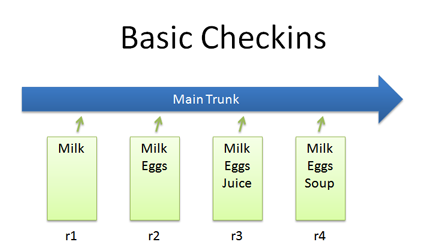
\includegraphics[scale=0.5]{images/basic_checkin.png}
\end{center}
Секогаш кога додаваме нова верзија, добиваме нова ревизија (r1, r2, r3, итн.).
\end{frame}

\begin{frame}[fragile]{Испраќање и модификување на датотека}{Checkins -
Subversion}
\begin{exampleblock}{Во Subversion :}
\begin{verbatim}
svn add list.txt
(modify the file)
svn ci list.txt -m "Changed the list"
\end{verbatim}
\end{exampleblock}
Знакот -m е пораката која се поставува за праќањето.
\end{frame}


    
\begin{frame}{Повлекување и менување}{Checkouts and Editing}
\begin{scriptsize}
Во реалноста, нема постојано потреба само од испрати (checking in) датотека.
Понекогаш треба да се повлече, промени и повторно испрати. Овој циклус изгледа
вака:
\end{scriptsize}
\begin{center}
    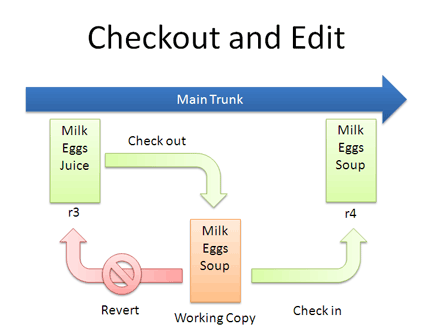
\includegraphics[scale=0.4]{images/checkout_edit.png}
\end{center}
\end{frame}

\begin{frame}[fragile]{Повлекување и менување}{Subversion}
\begin{scriptsize}
Ако не ви се допаѓаат промените и сакате да започнете одново, може да се вратите
(revert) на претходна верзија и да започнете одново (или да завршите). Кога
повлекувате, ја добивате последната (најновата) верзија. Ако сакате може да
ја назначите посакуваната ревизија.
\end{scriptsize}
\begin{exampleblock}{Во Subversion:}
\begin{verbatim}
svn co list.txt (get latest version)
...edit file...
svn revert list.txt (throw away changes)

svn co -r2 list.txt (check out particular version)
\end{verbatim}
\end{exampleblock}
\end{frame}

\begin{frame}{Разлики}{Diffs}
\begin{scriptsize}
Стеблото (trunk) чува историја на промени како што се менува датотеката.
Разликите се промените кои сте ги направиле при модификување: замислете дека
може да ги „излупите“ и да ги залепите на датотека.
\end{scriptsize}
\begin{center}
    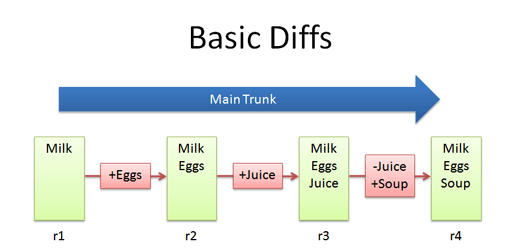
\includegraphics[scale=0.4]{images/basic_diffs.png}
\end{center}
\begin{scriptsize}
На пример, за да одиме од r1 на r2, додаваме (+Eggs). 
Замислете вадење на црвената лента и ставање на r1 за да се добие r2.\\ 
А за да се дојде од r2 до r3, додаваме Juice (+Juice). \\
За да дојдеме од r3 до r4, го острануваме Juice и додаваме Soup (-Juice,
+Soup).
\end{scriptsize}
\end{frame}

\begin{frame}[fragile]{Разлики}{Subversion}
\begin{scriptsize}
Повеќете системи за контрола на верзиите ги чуваат разликите наместо да чуваат
целосни копии на датотеките. Ова зачувува простор на дискот: 4 ревизии на една
датотека не значи дека имаме 4 копии. Имаме 1 копија и 4 мали разлики. 
\end{scriptsize}
\begin{exampleblock}{Во Subversion:}
\begin{verbatim}
svn diff -r3:4 list.txt
\end{verbatim}
\end{exampleblock}
\begin{scriptsize}
Разликите ни помагаат да ги забележиме промените („Како ја исправи таа грешка?“)
и да ги примениме од одна гранка на друга.\\
Прашање: Која е разликата од r1 до r4? 
\end{scriptsize}
\begin{exampleblock}{Решение}
\begin{verbatim}
+Eggs
+Soup
\end{verbatim}
\end{exampleblock}
\begin{scriptsize}
Забележете како “Juice“ воопшто не е вклучена - директниот скок од r1 на r4 нема
потреба од таа промена, затоа што Juice беше препокриена од Soup.
\end{scriptsize}
\end{frame}

\begin{frame}{Разгранување}{Branching}
Разгранувањата ни овозможуваат да ја ископираме содржината во посебен
директориум така што може да правиме измени одделно:
\begin{center}
    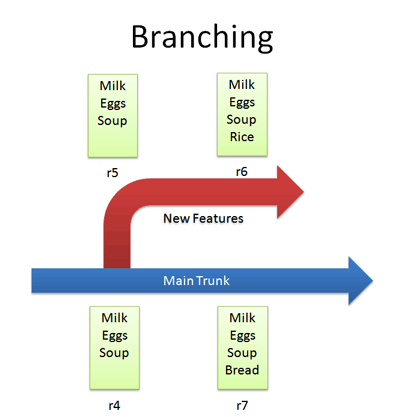
\includegraphics[scale=0.4]{images/first_branch.png}
\end{center}
\end{frame}

\begin{frame}{Разгранување}{Branching}
На пример, може да направиме гранка за нови, експериментални идеи за нашата
листа со нови состојки и рецепти. Во зависност од системот за
контрола на верзиите креирање на гранка (копија) може да го промени
бројот на ревизијата. Сега кога имаме нова гранка може да правиме
измени какви што сакаме. Заради тоа што сме на посебна гранка може да правиме
измени и тестови во изолација, знаејќи дека нашите измени нема никому да му
наштетат. А исто така и нашата гранка е под системот за контрола на верзиите.
\end{frame}

\begin{frame}[fragile]{Разгранување}{Subversion}
Во Subversion, гранка се креира со едноставно копирање на еден директориум во
друг.
\begin{exampleblock}{Во Subversion:}
\begin{verbatim}
svn copy http://path/to/trunk http://path/to/branch
\end{verbatim}
\end{exampleblock}
\begin{scriptsize}
Излегува дека разгранувањето и не така тежок концепт: едноставно копирање на
содржината во друг директориум. Веројатно сте го разграниле некој ваш школски
проект со копирање на безбедно место, за бидете сигурни дека имате „безбедна“
верзија на која може да се вратите ако нешто тргне лошо.
\end{scriptsize}
\end{frame}

\begin{frame}{Спојување}{Merging}
Разгранувањето изгледа едноставно, нели? Но, не е воопшто. \\
Одредување како ќе ги споиме промените од една гранка во друга може да биде
комплицирано.\\ 
Да речеме дека сакаме да го земе “Rice“ од нашата експериментална гранка во основната
гранка.\\
Како ќе го направиме ова?\\
Да ја додадеме разликата од r6 и r7 на основната гранка?\\ 
Грешка!\\
Ние сакаме да ги додадеме измените кои се случија во нашата гранка!\\
Тоа значи дека ја додаваме разликата на r5 и r6 на основната гранка.
\end{frame}

\begin{frame}{Спојување}{Merging}
\begin{center}
    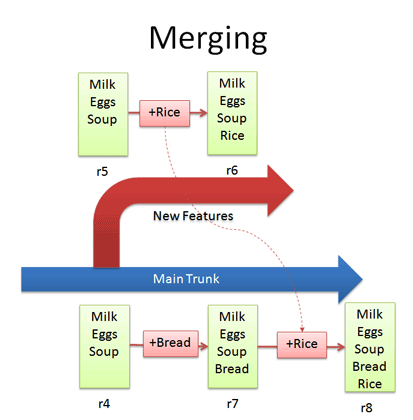
\includegraphics[scale=0.30]{images/merging.png}
\end{center}
\begin{scriptsize}
Ако ја додадевме разликата помеѓу r6 и r7, ќе го загубевме “Bread“ од основната
гранка. Ова е многу важно - замислете „лупење“ на промените на експерименталната
гранка (+Rice) и нивно додавање на основната. Основната може да имала и други
промени, што е во ред затоа што ние сакаме само да го додаеме “Rice“.
\end{scriptsize}
\end{frame}

\begin{frame}[fragile]{Спојување}{Subversion}
Во Subversion, спојувањето е многу слично на разликите. Во основното
стебло изврешете ја командата:
\begin{exampleblock}{Во Subversion:}
\begin{verbatim}
svn merge -r5:6 http://path/to/branch
\end{verbatim}
\end{exampleblock}
\begin{scriptsize}
Оваа команда прави разлика на r5-r6 од експерименталното стебло и ги применува
на тековната локација. За жал, Subversion нема начин за едноставно следење на
кои спојувања се извршени, така што ако не сте внимателни може да ги направите
истите промени два пати.
\end{scriptsize}
\end{frame}


\begin{frame}{Конфликти}{Conflicts}
Мнгоу пати, системите за контрола на верзии автоматски ги спојуваат измените во
различни делови од датотеката. Конфликти се појавуваат кога овие автоматски
спојувања не може да се направат затоа што промените се контрадикторни.\\
Јован сака да ги извади јајцата и да ги замени со сирење (-eggs, +cheese), но
Суза сака да ги замени јајцата со ход дог (-eggs, +hot dog).
\end{frame}

\begin{frame}{Конфликти}{Conflicts}
\begin{center}
    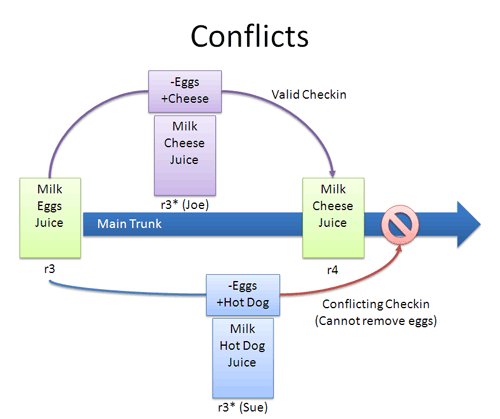
\includegraphics[scale=0.4]{images/vcs_conflict.png}
\end{center}
\end{frame}

\begin{frame}[shrink=10]{Конфликти}{Разрешување}
Во овој момент сме во трка: ако Јоаван ги испрати промените прв, тоа е промената
која ќе се направи (а Суза не може да ја направи својата промена).
\linebreak
Кога промените се поклопуваат и се контрадикторни како во овој случај, системот
за контрола на верзии може да јави конфликт и да не ви дозволи да ги испратите
промените. На вас е оставено да одлучите која нова верзија ќе ја оставите и како
ќе ја разрешите оваа дилема. Неколку пристапи се можни:
\begin{itemize}
  \item \textbf{Применете ги вашите измени.} Синхронизирајте се со најновата верзија r4 и
  применете ги вашите измени на оваа датотека: Додадете го хот дог во листата
  која што веќе има сирење.
  \item \textbf{Препокриете ги нивните измени со вашите.} Повлечете ја најновата
  верзија (r4), копирајте ја врз вашата верзија и испратете ја вашата верзија.
  Како ефект, ова го отстранува сирењето и го заменува со хот дог.
\end{itemize}
Конфликтите се ретки но може да бидат проблематични. Вообичаено ја повлекувате
најновата верзија и ги применувате вашите измени врз неа.
\end{frame}

\begin{frame}{Тагирање}{Tagging}
Многу системи ви овозможуваат да ги тагирате (означите) ревизиите за едноставно
референцирање. На овој начин може да се референцирате на „Верзија 1.0“ наместо
на генерираниот број.
\begin{center}
    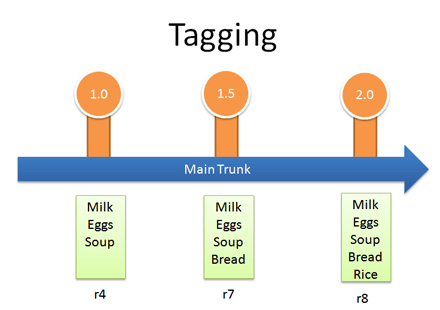
\includegraphics[scale=0.4]{images/tagging.png}
\end{center}
\end{frame}

\begin{frame}[fragile]{Тагирање}{Subversion}
Во Subversion, таговите се едноставни стебла кои се сложувате да не ги
менувате. Тие се овде само за потомство, за да може да видите што точно
содржела вашата верзија 1.0. Така овие стебла завршуваат тука и не се спојуваат.
\begin{exampleblock}{Во Subversion:}
\begin{verbatim}
(in trunk)
svn copy http://path/to/revision http://path/to/tag
\end{verbatim}
\end{exampleblock}
\end{frame}

\begin{frame}{Реален пример}{Managing Windows Source Code}
Претпоставивме дека Windows се управува преку споделен директориум, но тоа не
така. Па тогаш како е?\\
Постои основна линија со стабилни верзии на Windows. Секоја група (Networking,
User Interface, Media Player, инт.) има свое стебло за да развива нови
функционалности. Овие стебла се под развој и се помалку стаблини од основната.
Вие развивате нови функционалности и ги интегрирате превртено “Reverse Integrate
(RI)” во основната линија. Подоцна, се интегрирате нормално “Forward Integrate”
и ги добивате последните промени од основната линија во вашето стебло.
\end{frame}

\begin{frame}{Реален пример}{Managing Windows Source Code}
\begin{center}
    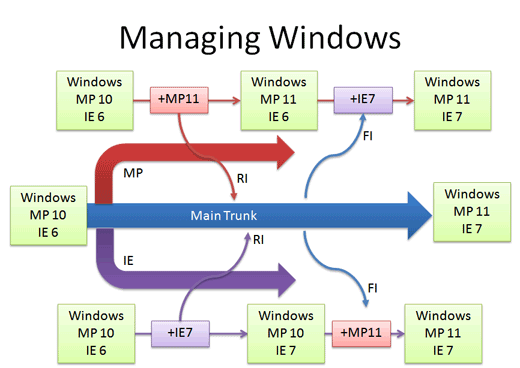
\includegraphics[scale=0.4]{images/windows.png}
\end{center}
\end{frame}

\begin{frame}[shrink=10]{Реален пример}{Managing Windows Source Code}
Да речеме дека сме во Media Player 10 и IE 6. Тимот на Media Player прави
верзија 11 во нивното стебло. Кога е готова верзијата, постои додаток од 10 - 11
кој се применува на основното стебло (исто како во примерот со “Rice“ само
малку покомплицирано). Ова е свртена интеграција од гранка во стебло. Тимот на
IE го прави истото нешто.
\linebreak
Подцна, тимот Media Player може да го собере најновиот код од други тимови, како
IE. Во овој случај, Media Player се интегрира нормално и ги зема најновите
додатоци од основнато стебло во нивната гранка. Ова е како повлекување на
“Bread” во експерименталното стебло, само повторно, малку покомплицирано.
\linebreak
Во реалноста, постојат многу слоеви на стебла и под-стебла, заедно со метрики на
квалитетот за утврдување дали може да се случи интеграцијата.
Основната идеја е дека: стеблата помагаат да се \textbf{управува со
комплексноста}.\\
И така се запознавме како е организиран еден од најголемите софтверски
 проекти :)
\end{frame}

\section{Заклучок}

\begin{frame}{Заклучок}
Основна цел на овој час беше основно запознавање на повисоко ниво со системите
за контрола на верзии.
Основни заклучоци се:
\begin{itemize}
  \item \textbf{Употребувајте системи за контрола на верзии.}
  \item \textbf{Започнете полека да го употребувате}
  \item \textbf{Продолжете да учите}
\end{itemize}
\end{frame}

\begin{frame}{Материјали}{}
	Предавања, аудиториски вежби, соопштенија\\
	\href{http://courses.finki.ukim.mk/}{\textbf{courses.finki.ukim.mk}}
	\vfill
	{\Huge Прашања ?}
\end{frame}

\end{document}
